%!TEX root = ../main.tex

%%%%%%%%%%%%%%%%%%%%%%%%%%%%%%%
%%%%%%%%%%%%%%%%%%%%%%%%%%%%%%%
\chapter{Theoretical basics}
\label{chap:theoretical}

The following theoretical basics are summarized from the standard literature in optics \autocite{bornPrinciplesOpticsElectromagnetic1999,hechtOptik2005,lipsonOptik1997,niedrigOptikWellenUnd2004} and more specifically Raman application \autocite{herzbergMolecularSpectraMolecular2013,schraderInfraredRamanSpectroscopy1995}. In addition the given handbook \autocite{klevanskyTDLASTunableLaser2021} is used as well.

The central principle TDLAS relies on, is the absorption of light. Next to absorption there are more processes which can occur with an incoming photon or light beam, such as scattering, reflection, or diffraction. In this case the focus is only on the first. Absortion of photons, or electromagnetic radiation, can only occur, if the struck molecule matches the energy of the photon with the energy difference of two of its discrete energy levels. This is called the resonance condition. This energy can be expressed as
\begin{align}
    E=h \cdot v \nonumber .
\end{align}
The absorbtion can be visualized when hitting the molecule with a bandwith light source. When analyzing the spectrum after the interaction, there are gaps or narrow dark bars occuring in the spectrum. Smaller molecules tend to form discrete lines, larger molecules more washed out reduction of the light spectrum. When using lower enrgy containing infrared radiation (IR), more vibrational or rotational states in the electronic ground state of the molecule are penetrated. In comparison the usage of higher energy contain ultra violet light, the electonic ground state can be elevated as well, and other unwanted effects such as flourescense can occur. With the IR absorption, the generated spectrum and its gaps are acting like a fingerprint for the molecule. Species determination is easily possible that way.

% The interpretation of the gathered absorbtion signals, resp. the understanding of the quantitative and qualitative meaning, is further elaborated in \autoref{sec:strategy}.

\begin{figure}[!htb]
    \centering
    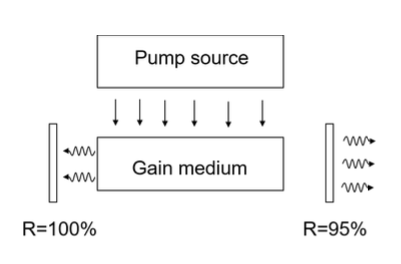
\includegraphics[width=.5\textwidth]{02kapitel/laser-simple.png}
    \caption[Components and working pronciples of a laser]{Simple working principle of a laser; simplificated components \autocite{klevanskyTDLASTunableLaser2021}}
    \label{fig:laser-simple}
\end{figure}

To precisely analyse the absorption spectra, a bandwith light source is not pleasent to use. A better way is the usage of a wavelength tunable laser. This can e.g. be achieved with a Littrow laser arrangement (see \autoref{fig:littrow-laser}), like in this experiment. This arrangement allows a tunable output wavelength through a variable placement of a grating, thus realised through an easy to control electrical motor. The diffraction grating reflects the first diffraction order of the laser beam back and forms a standing wave. It is used with its easy positioning for creating the needed amplification (the basic laser principle is sketched in \autoref{fig:laser-simple}). After reaching the laser threshold, the laser beam is coupled into a glass fibre and guided to the experimental setup. As a pump source a laser diode is utilized. The emitted basis wavelength is further tunable through the diode current and the temperature.

\begin{figure}[!htb]
    \centering
    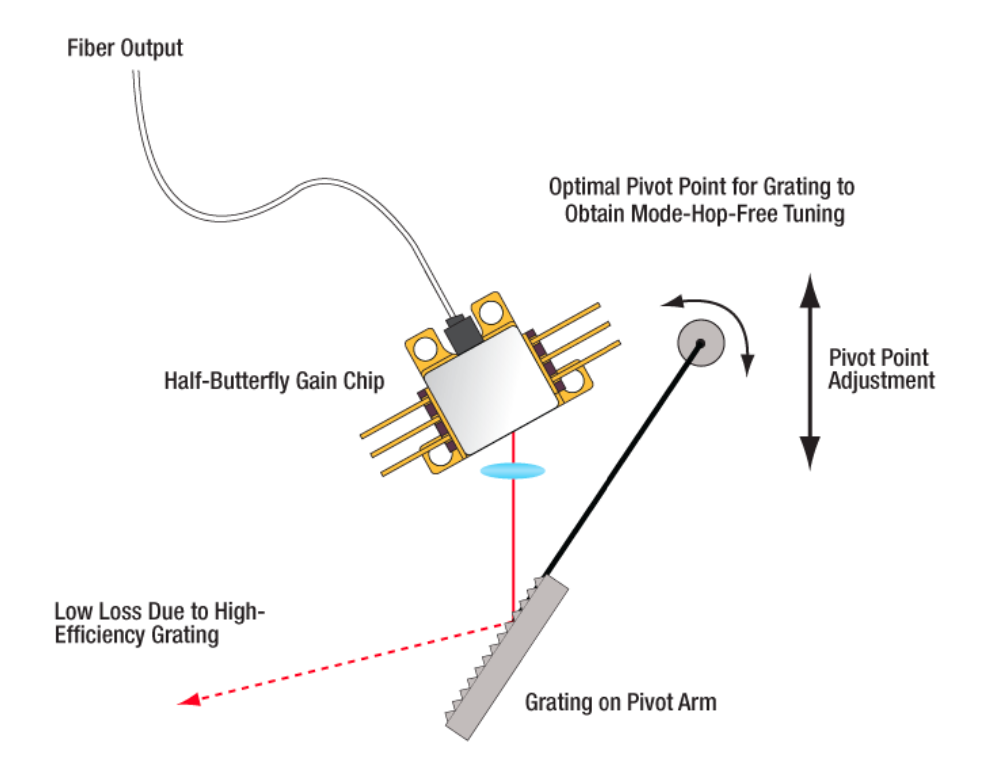
\includegraphics[width=.7\textwidth]{02kapitel/littrow-laser.png}
    \caption[Tunable littrow laser arrangement]{Tunable littrow laser arrangement \autocite{klevanskyTDLASTunableLaser2021}}
    \label{fig:littrow-laser}
\end{figure}

%%%%%%%%%%%%%%%%%%%%%%%%%%%%%%%
%%%%%%%%%%%%%%%%%%%%%%%%%%%%%%%
\chapter{Experimental setup}
\label{chap:experimental}

% Following chapter shall describe the used experimental setup, the preparations before the measurements, the possible expectations and outcomes of the test and observations during the experiment. The strategy of the data evaluation and result calculation shall be explained.
Following chapter shall describe the used experimental setup. The strategy of the data evaluation and result calculation shall be explained.

%%%%%%%%%%%%%%%%%%%%%%%%%%%%%%%
\section{Measurement setup and preparations}
\label{sec:setup}

A scheme of the measurement setup is illustrated in \autoref{fig:experimental-setup}. Controlling the whole setup, mainly the Littrow laser system and the chopper, and reading out the oszilloscope for data saving, is a computer. The laser signal is generated with a tunable diode laser setup (see \autoref{fig:littrow-laser}) for generating a defined bandwith (between $1891~\mathrm{nm}$ and $2022~\mathrm{nm}$) of wavelengths (see \autoref{chap:theoretical} for a functional description). This signal is split into two beams and measurement paths. The chopper is acting as a pulser, so that the substance molecules and the photo diodes can relax and deexcite between the absortion processes. Between the chopper and the photodiode the probe is placed. After an intensification of the signal, it is read out with an oszilloscope. As a consequence the measurement is transmittive. 

\begin{figure}[!htb]
    \centering
    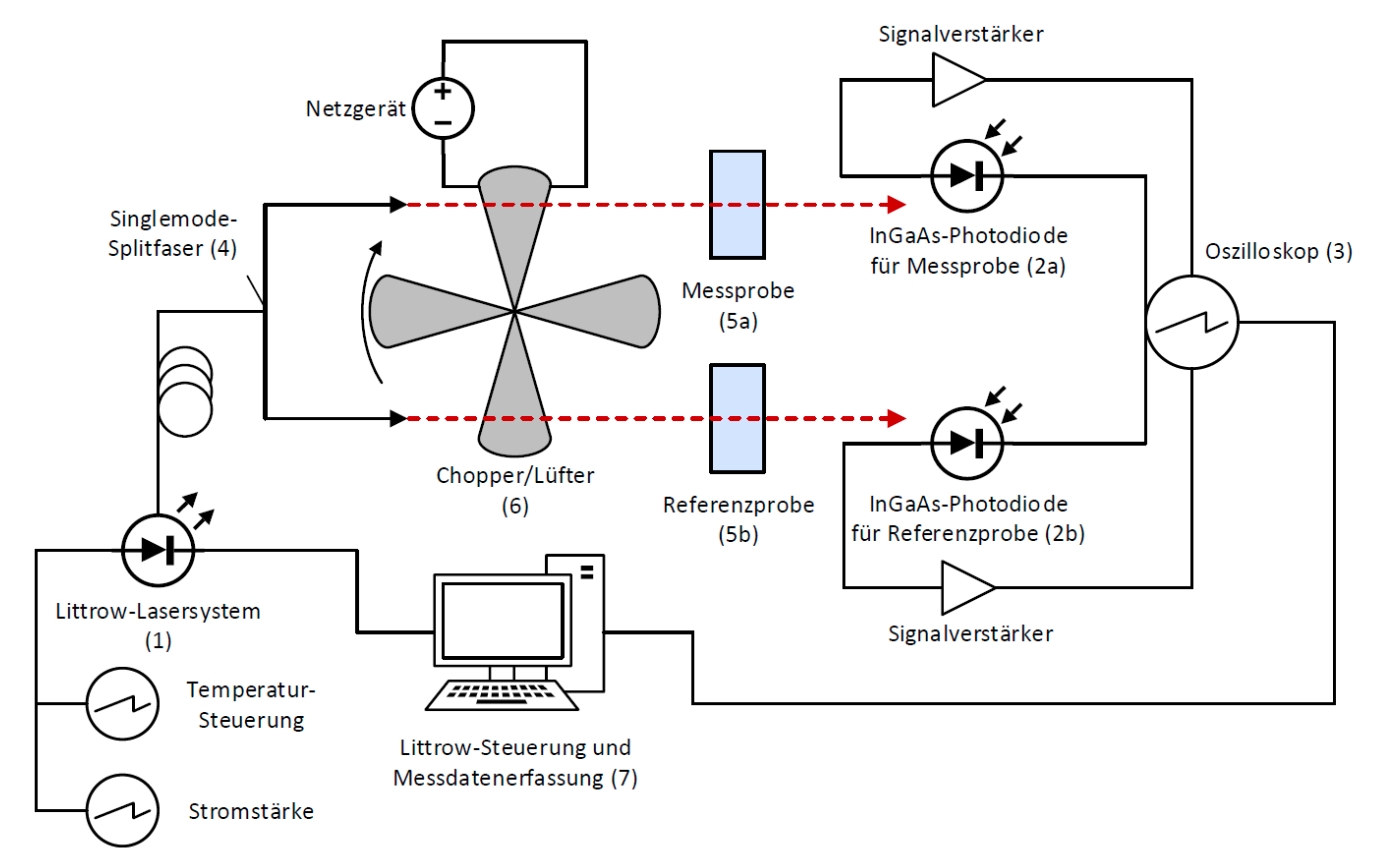
\includegraphics[width=\textwidth]{02kapitel/measurement_setup.png}
    \caption[Experimental setup of the TDLAS measurement]{Experimental setup of the TDLAS measurement \autocite{klevanskyTDLASTunableLaser2021}}
    \label{fig:experimental-setup}
\end{figure}

The procedure of the measurement is like following, whereas the laboratory script \autocite{klevanskyTDLASTunableLaser2021} is giving more detailed information.

\begin{enumerate}
    \item Starting up sequence
    \enumeratext{
        For starting up the experiment, the laptop has to be boot up and the necessary software has to be started. Further, the control devices and operating temperatures have to be checked, such as laser temperature, laser current and voltage supply.
    }
    \item Calibration of the two measurement channels
    \enumeratext{
        Cuvettes have to be removed and a calibration measurement at each wavelength over both measurement paths A and B is needed. The calibration factor KF is calculated to normalize both signal pathways (especially the photodiodes). This step makes both pathways comparable.
    }
    \item Absorption spectrum measurement
\end{enumerate}
As last step, the actual measurement of both species is carried out. Pathway A is used for aquiring the absortion spectrum of the species, path B is used with an emty cuvette as a reference measurement. Important to note is the dark signal of both channels.
\vspace{12pt}

%%%%%%%%%%%%%%%%%%%%%%%%%%%%%%%
\section{Post-processing strategy}
\label{sec:strategy}

% \commenting{
%     \begin{itemize}
%         \item calibration factor KF (channels to each other)
%         \item absorption spectra vs empty cuvette reference (normalize with KF; difference between them are the intensities of the absorbed signals)
%         \item wavelegths for extinction coefficient determination
%         \item calculation of extinction coefficient
%         \item possible uncertainties and errors
%     \end{itemize}
% }

Starting off with the raw signals from the A/D-converter, the signal has to be corrected and normalized. Due to knwon and discussed effects of dark signals and different signal intensities from photo diodes, e.g. from differences out of manufacturing, two calibration steps have to be carried out. The dark signal must be substracted from the general intensity (following \autoref{eq:intensity}), the two channels have to be calibrated to each other with the help of an wavelength dependent calibration factor $KF$ (see \autoref{eq:calibration}).
\begin{align}
    I_\mathrm{measurement}&=I_\mathrm{photodiode}+I_\mathrm{dark} \label{eq:intensity} \\[12pt]
    KF(\lambda)&=\frac{I(\lambda)}{I_\mathrm{0}(\lambda)} \label{eq:calibration}
\end{align}
The calibration has to be considered for each discrete wavelength, the dark signal is uniformly relevant over the complete spectrum.

\begin{figure}
    \centering
    \vspace{12pt}
    \begin{tikzpicture}%[every node/.style={rectangle, draw, align = center, rounded corners=5pt, minimum height=24pt, font=\footnotesize}]
        % nodes
        \node [papData]                                      (signal)    {measurement signals A and B};
        \node [papProcess, below of = signal, yshift=-10mm]  (corr)      {dark correction};
        \node [papData, left = of corr]                      (dark)      {dark signal};
        \node [papProcess, below of = corr, yshift=-5mm]     (kf)        {calibration with factor $KF(\lambda)$};
        \node [papData, left = of kf]                        (calib)     {calibration signal};

        \node [papProcess, right = of kf]                    (ext-calc)  {extinction calculation for each $\lambda$};
        \node [papData, above of = ext-calc, yshift=5mm]     (lambda)    {$\lambda=[...]$};
        \node [papEnd, below of = kf, yshift=-10mm]          (abs)       {absorption spectra $A(\lambda)$};
        \node [papEnd, right = of abs]                       (ext)       {extinction coefficient(s) $\epsilon(\lambda)$};

        % pathways
        \path [papLine] (dark) -- (corr);
        \path [papLine] (calib) -- (kf);
        \path [papLine] (signal) -- (corr);
        \path [papLine] (corr) -- (kf);
        \path [papLine] (kf) -- (ext-calc);
        \path [papLine] (lambda) -- (ext-calc);
        \path [papLine] (ext-calc) -- (ext);
        \path [papLine] (kf) -- (abs);

    \end{tikzpicture}
    \vspace{6pt}
    \caption{Evaluation procedure diagram}
    \label{fig:scheme-eval}
\end{figure}

Since the Transmission ratio $T$, depending on the laser shot intensity $I_\mathrm{0}$ and the transmitted intensity $I$ is given through 
\begin{align}
    T=\frac{I}{I_\mathrm{0}} \nonumber
\end{align}
and the Absorption ratio with the substraction of $T$ from one, we can state:
\begin{align}
    A=1-\frac{I}{I_\mathrm{0}} \nonumber
\end{align}
Further taking into account both calibration steps, we can develop as Absorption spectra
\begin{align}
    A(\lambda)=1-\frac{(I_\mathrm{A} - I_\mathrm{dark}) \cdot KF(\lambda)}{I_\mathrm{B} - I_\mathrm{dark}} \label{eq:absorption-spectrum}.
\end{align}
Determing the extinction coefficient is possible through rearrangeing Lambert-Beer's law (see \autoref{eq:lambert-beer-rearranged}). IMportant to note is the wavelength and temperature dependency of this coefficient, although the last one is kept constant at this experiment. Selected for evaluation of $\epsilon(\lambda)$ are follwing wavelenghts:
\begin{align}
    \lambda&=[1906, 1950, 1977, 2003]~\mathrm{nm} \nonumber \\[6pt]
    \epsilon(\lambda)&=\frac{log(I_\mathrm{0})-log(I)}{c \cdot d} \label{eq:lambert-beer-rearranged}
\end{align}
The evaluation procedure is shown in \autoref{fig:scheme-eval}. For this calculation following parts have to be recorded during the experiment:
\begin{enumerate}
    \item Measurement signal of the species at every wavelength
    \item Reference spectrum at every wavelength
    \item Dark signal before the measurement
    \item Simultaneous signal of path A and B at every wavelength
\end{enumerate}

%%%%%%%%%%%%%%%%%%%%%%%%%%%%%%%
%%%%%%%%%%%%%%%%%%%%%%%%%%%%%%%
\chapter{Results}
\label{chap:results}

%%%%%%%%%%%%%%%%%%%%%%%%%%%%%%%
\section{Data presentation and preparation}

%%%%%%%%%%%%%%%%%%%%%%%%%%%%%%%
\section{Evaluation}

%%%%%%%%%%%%%%%%%%%%%%%%%%%%%%%
\section{Error discussion}